\documentclass[a4paper, 12pt]{article}

%Абзацный отступ

\usepackage{indentfirst}

%Рисунки

\usepackage{subfig}
\usepackage{graphicx}
\usepackage{wrapfig}

%Гиперссылки и работа с цветом

\usepackage{hyperref}
\usepackage[rgb]{xcolor}
\hypersetup{			%Гиперссылки
	colorlinks=true, 	%false: ссылки в рамках
	urlcolor=blue		%на URL
}

%Русский язык

\usepackage[T2A]{fontenc}		%кодировка
\usepackage[utf8]{inputenc}		%кодировка исходного текста
\usepackage[english, russian]{babel}	%локализация и переносы


%Математика

\usepackage{amsmath, amsfonts, amssymb, amsthm, mathtools, mathrsfs}

%Пакет с градусом

\usepackage{gensymb}


\author{Штрайх Роберт}
\title{Работа 4.3.3. Исследование разрешающей способности микроскопа методом Аббе}
\date{09 февраля 2022 г.}

\begin{document}
\begin{titlepage}
	\centering
	\vspace{5cm}
	{\scshape\LARGE Московский физико-технический институт \par}
	\vspace{4cm}
	{\scshape\Large Лабораторная работа №4.3.3 \par}
	\vspace{1cm}
	{\huge\bfseries Исследование разрешающей способности микроскопа методом Аббе\par}
	\vspace{1cm}
	\vfill
\begin{flushright}
	{\Large выполнил студент 006 группы ФЭФМ}\par
	\vspace{0.3cm}
	{\Large Штрайх Роберт}
\end{flushright}
	

	\vfill

% Bottom of the page
	Долгопрудный, 2022 г.
\end{titlepage}

\newpage

\textbf{Цель работы:} определение дифракционного предела разрешения объектива микроскопа методом Аббе

\textbf{В работе используются:} лазер; кассета с набором сеток разного периода; линзы; щель с микрометрическим винтом; оптический стол с набором рейтеров и крепежных винтов; экран; линейка.

\section*{Теоретическое введение}

Всякая оптическая система, предназначенная для получения изображений, имеет конечный
предел разрешения, т.е. ограниченную возможность раздельного наблюдения близко расположенных
предметов. Принципиальной причиной, ограничивающей предел разрешения, является дифракция
световых волн. Разрешающей способностью оптического прибора называют минимальное
расстояние $l_{min}$ между двумя точками в пространстве предметов, которое прибор может
разрешить.
Для иммерсионного микроскопа (объект находится в иммерсионной среде жидкости с показателем
преломления $n$) разрешающая способность объектива при некогерентном освещении:

\[l_{min} \approx \dfrac{0.61\lambda}{n~\sin A},\]

где $A$ - апертурный угол объектива микроскопа. 

\begin{figure}[h]
\begin{center}
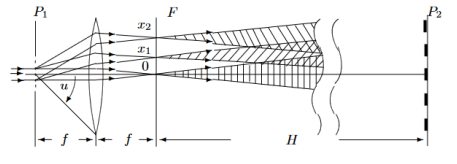
\includegraphics[width=1\textwidth]{Pic1.png}
\end{center}
\caption{Образование изображения в объективе микроскопа.} \label{Образование изображения}
\end{figure}

Рассмотрим теперь когерентно освещённый объект, наблюдаемый в микроскоп. Схема образования
изображения в объективе микроскопа представлена на рис. \ref{Образование изображения}. Для простоты рассмотрим случай,
когда предметом является периодическая структура (дифракционная решётка), освещаемая
параллельным пучком лучей. При наблюдении в микроскоп предмет располагается вблизи переднего
фокуса объектива. При освещении решётки волнами, наклонными к оси, с углом наклона чуть
меньшим апертуры $A$ волны нулевого порядка сфокусируются на край диафрагмы. Для получения
изображения достаточно, чтобы на противоположные края сфокусировались волны 1-го порядка,
т. е. угол между волнами 0 и 1 порядка должен быть равен $2A$. Минимальное разрешаемое объективом расстояние определяется условием:

\begin{equation} \label{l_min}
l_{min}\approx\dfrac{\lambda}{\sin A}\approx\dfrac{\lambda}{D/2f},
\end{equation}

где $D$ - диаметр диафрагмы. При этом диафрагма, расположенная симметрично, пропускает нулевой и $\pm 1$ дифракционные максимумы.

В нашей работе применяется двумерная решётка сетка. Её можно рассматривать как две
скрещенные (перпендикулярные друг к другу) решётки. Узкий пучок монохроматического света,
пройдя через решётку с вертикальными штрихами, даёт совокупность максимумов, расположенных
вдоль горизонтальной линии. Световой пучок, соответствующий каждому максимуму, проходя через
вторую решётку, распадается на новую совокупность световых пучков, дающих максимумы вдоль 
вертикальной линии. Главные максимумы возникают тогда, когда одновременно выполняются
условия:  

\begin{equation} \label{Главные максимумы}
d\sin\theta_x = m_x\lambda, ~~~ d\sin\theta_y = m_y\lambda,
\end{equation}

где $m_x$ и $m_y$ - целые числа, характеризующие порядки дифракционных максимумов, $\theta_x$ и $\theta_y$ - направления на главные дифракционные максимумы в горизонтальной и вертикальной плоскостях соответственно.

\begin{figure}[h]
\begin{center}
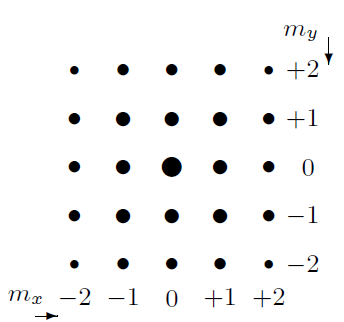
\includegraphics[width=0.3\textwidth]{Pic2.png}
\end{center}
\caption{Дифракция Фраунгофера на двумерной решётке (сетке).} \label{Дифракция}
\end{figure}

Максимумы, удовлетворяющие условию $\theta_x$, $\theta_y < u$, создают в задней фокальной плоскости $F$
объектива картину дифракции Фраунгофера (рис. \ref{Дифракция}) первичное изображение. Если теперь
поместить в фокальной плоскости вертикальную щель так, чтобы через неё проходили
дифракционные максимумы с $m_x = 0$ и $m_y = 0, \pm 1, \pm 2, ... ,$ то в плоскости $P_2$ получится
изображение решётки с горизонтально расположенными штрихами. Если, наоборот, пропустить
максимумы с $m_y = 0$ и $m_x = 0, \pm 1, \pm 2, ... ,$ то в $P_2$ получится изображение решётки с вертикальными
штрихами. Таким образом можно продемонстрировать явление пространственной фильтрации --
выделение различных структур в изображении.

\section*{Экспериментальная установка}

Схема модели проекционного микроскопа представлена на рис. \ref{Установка}. Предметом служат сетки, расположенные в кассете. Смена сеток осуществляется поворотом внешнего кольца кассеты.

\begin{figure}[h]
\begin{center}
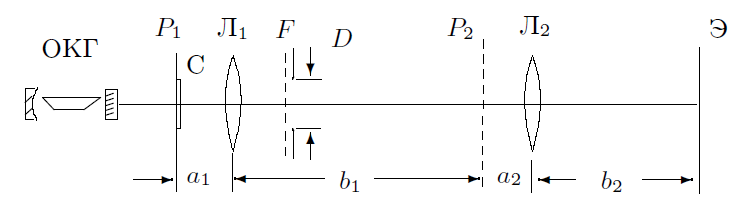
\includegraphics[width=1\textwidth]{Pic3.png}
\end{center}
\caption{Схема экспериментальной установки -- модель проекционного микроскопа.} \label{Установка}
\end{figure}

\section*{Ход работы}

\subsection*{Определение периода решёток по их пространственному спектру}

Определим расстояния между соседними дифракционными максимумами путем измерения расстояния между удалёнными друг от друга максимумами (горизонтальными или вертикальными) и числа промежутков между ними.

Длина волны лазера $\lambda = 532$ нм, расстояние от сетки до экрана $H = 114$ см. 

Период решеток найдем по формулам \eqref{Главные максимумы}.

Угол мал:

\[\sin\theta_{x,y}\approx \theta_{x,y}\approx m_{x,y}\dfrac{l}{H}\]

Погрешности $H$, $l$: $\sigma_H = \sigma_l = 0.5$ мм

$\theta$: $\dfrac{\sigma_{\theta}}{\theta} = \sqrt{\left(\dfrac{\sigma_l}{l}\right)^2 + \left(\dfrac{\sigma_H}{H}\right)^2}$


$d$: $\dfrac{\sigma_d}{d} = \dfrac{\sigma_{\theta}}{\theta}$

\begin{table}[h!] \label{Tab1}
\centering
\begin{tabular}{|l|l|l|l|l|l|}
\hline
N сетки & l, мм & $\theta \cdot 10^3$ & $\sigma_{\theta} \cdot 10^3$ & d, мкм & $\sigma_d$, мкм \\ \hline
1       & 36,7  & 32,2                    & 0,4 & 16,5   & 0,2 \\ \hline
2       & 24    & 21,1                    & 0,4 & 25,2   & 0,5 \\ \hline
3       & 12    & 10,5                    & 0,4 & 50,7   & 1,9 \\ \hline
4       & 6     & 5,3                     & 0,4 & 100,4  & 7,6 \\ \hline
5       & 4,5   & 3,9                     & 0,4 & 136,4  & 13,9 \\ \hline
\end{tabular}
\caption{Периоды решеток (пространственный спектр)}
\end{table}

\subsection*{Определение периода решеток по изображению, увеличенному с помощью модели микроскопа}

\begin{table}[h!] \label{Tab2}
\centering
\begin{tabular}{|l|l|l|l|l|l|}
\hline
$a_1$, мм & $a_2$, мм & $b_1$, мм & $b_2$, мм & $f_1$, мм & $f_2$, мм \\ \hline
160    & 27     & 773    & 315    & 110    & 25     \\ \hline
\end{tabular}
\caption{Характерные размеры}
\end{table}

$\sigma_{a_1} = \sigma_{b_1} = \sigma_{b_2} =0.5$ мм, $\sigma_{a_2} = 0.004$ мм,
\[a_2 = \dfrac{b_2 f_2}{b_2 - f_2}\]
\[\sigma_{a_2} = \dfrac{f_{2}^2}{(b_2 - f_2)^2} \sigma_{b_2}\]

Увеличение системы $\dfrac{b_1b_2}{a_1a_2} = 56.36$. Истинные периоды сетки связаны с периодами изображения соотношением:

\[d = \dfrac{a_1a_2}{b_1b_2} l\]

$\sigma_r = 0.5$ мм, $r$ -- расстояние между двумя максимумами,

$r = nl$, $l$ -- период изображения сетки, $n$ -- число максимумов

$\sigma_l = \dfrac{\sigma_r}{r}l$, $\sigma_d = d \sqrt{(\dfrac{\sigma_{a_1}}{a_1})^2+(\dfrac{\sigma_{a_2}}{a_2})^2+(\dfrac{\sigma_{b_1}}{b_1})^2+(\dfrac{\sigma_{b_2}}{b_2})^2+(\dfrac{\sigma_l}{l})^2}$

\begin{table}[h!] \label{Tab3}
\centering
\begin{tabular}{|l|l|l|l|l|l|l|}
\hline
N сетки & l, мм & d, мкм & r, мм & n & $\sigma_l$, мм & $\sigma_d$, мкм \\ \hline
1       & 1,7   & 30,2   & 10    & 6 &            0,1 &      1,8        \\ \hline
2       & 2,5   & 44,4   & 20    & 8 &            0,1 &       1,8       \\ \hline
3       & 5     & 88,7   & 30    & 6 &            0,1 &        1,8      \\ \hline
4       & 10    & 177,4  & 40    & 4 &            0,1 &         1,9     \\ \hline
5       & 13,3  & 236    & 40    & 3 &            0,2 &          3,6    \\ \hline
\end{tabular}
\caption{Периоды решеток (изображение, увеличенное микроскопом)}
\end{table}

\subsection*{Определение периодов решеток по оценке разрешающей способности микроскопа}

Определим для каждой решетки минимальный размер диафрагмы $D$, при котором на экране еще видно изображение сетки (при меньших размерах щели изображение -- одномерная решетка). Погрешность $\sigma_D  = 5$ мкм. Минимальное расстояние (период решетки d) рассчитаем по формуле \eqref{l_min}. Погрешность $\sigma_d = d \dfrac{\sigma_D}{D}$.

\begin{table}[h!] \label{Tab4}
\centering
\begin{tabular}{|l|l|l|l|}
\hline
N сетки & D, мкм & d, мкм & $\sigma_d$, мкм \\ \hline
3       & 600   & 44,3   & 0,4 \\ \hline
4       & 336    & 79,2  & 1,2 \\ \hline
5       & 182   & 145,4   & 4,0 \\ \hline
\end{tabular}
\caption{Периоды решеток (разрешающая способность микроскопа)}
\end{table}

\begin{figure}[h!]
\begin{center}
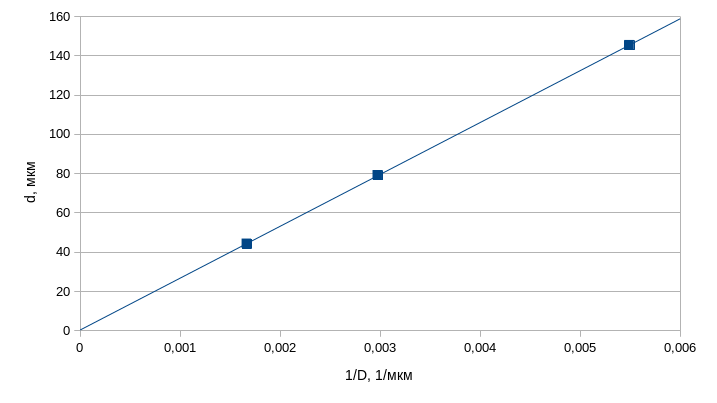
\includegraphics[width=1\textwidth]{График.png}
\end{center}
\caption{$d = f(1/D)$} \label{График}
\end{figure}

\newpage
\subsection*{Пространственная фильтрация и мультиплицирование}

\subsubsection*{Пространственная фильтрация}

В эксперименте с пространственной фильтрацией использовалась 4 сетка.

\begin{figure}[h!]
\begin{center}
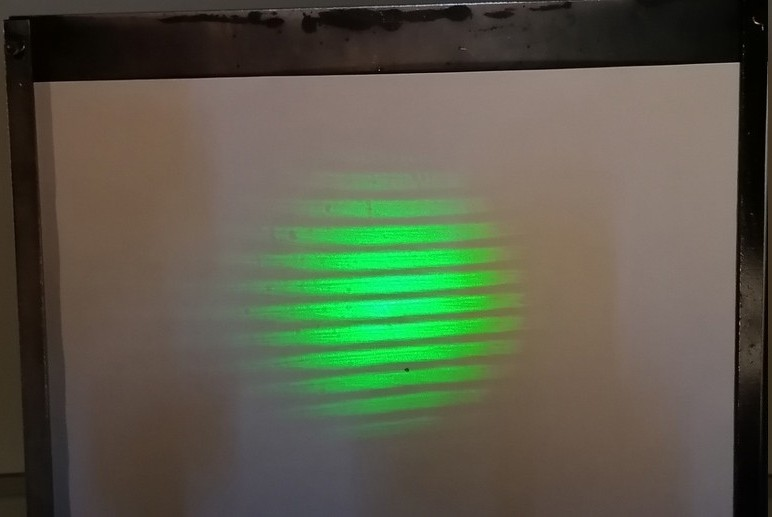
\includegraphics[width=1\textwidth]{Горизонтальный.jpg}
\end{center}
\caption{Вертикальное положение щели (0,$m_x$)} \label{Горизонтальные полосы}
\end{figure}

\begin{figure}[h!]
\begin{center}
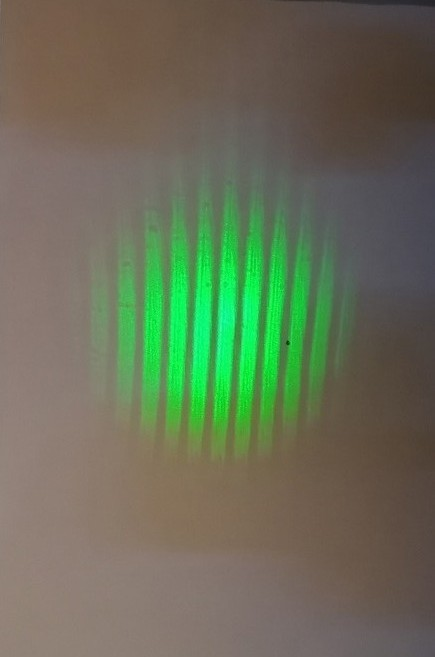
\includegraphics[width=0.75\textwidth]{Вертикальные.jpg}
\end{center}
\caption{Горизонтальное положение щели ($m_y$, 0)} \label{Вертикальные полосы}
\end{figure}

\begin{figure}[h!]
\begin{center}
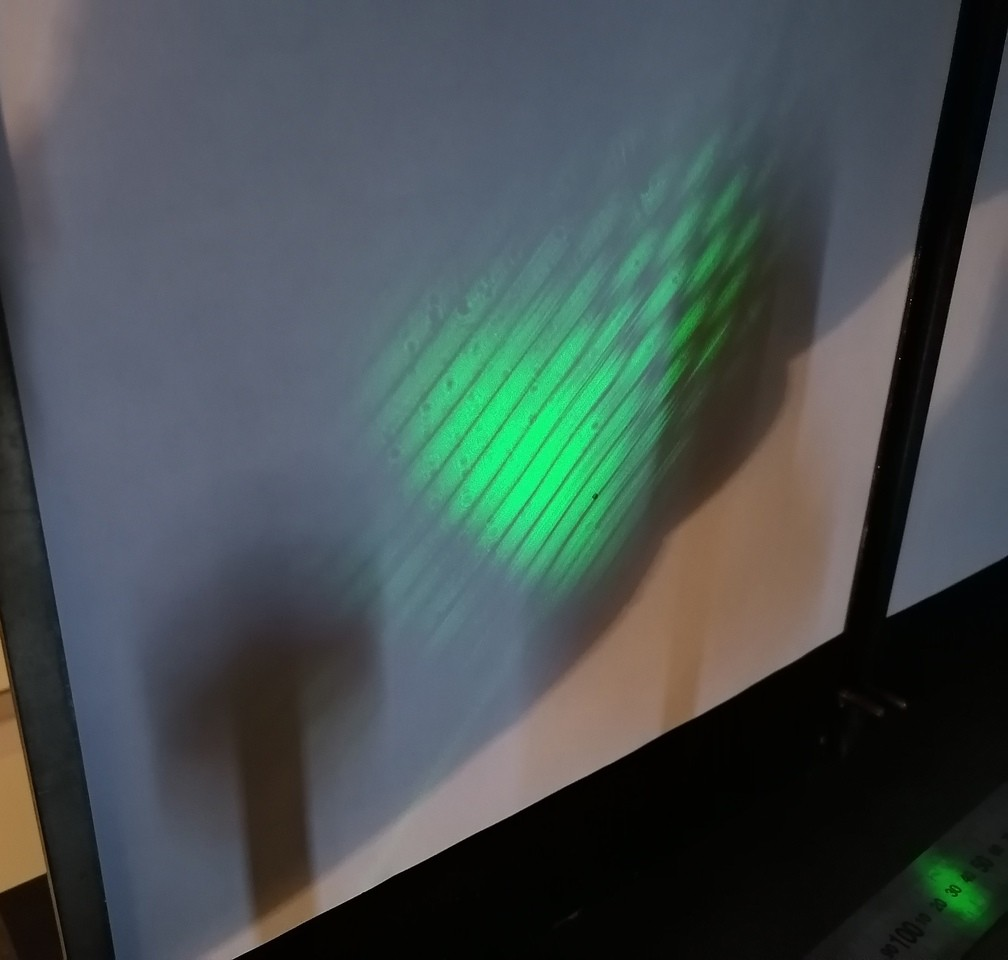
\includegraphics[width=1\textwidth]{45_градусов.jpg}
\end{center}
\caption{Положение щели под углом 45$\degree$, $m_x=m_y$} \label{45}
\end{figure}

\clearpage
\subsubsection*{Мультипликация}

Для наблюдения эффекта мультиплицирования поставим сетку впереди диафрагмы.

1.Оставим размер щели неподвижным, меняем сетки:

\begin{figure}[h!]
\begin{center}
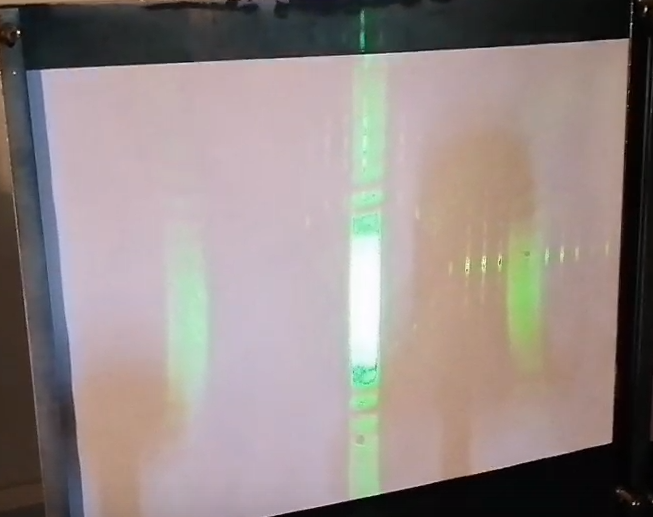
\includegraphics[width=1\textwidth]{Сетка3.png}
\end{center}
\caption{Сетка №3} \label{Сетка-3}
\end{figure}

\begin{figure}[h!]
\begin{center}
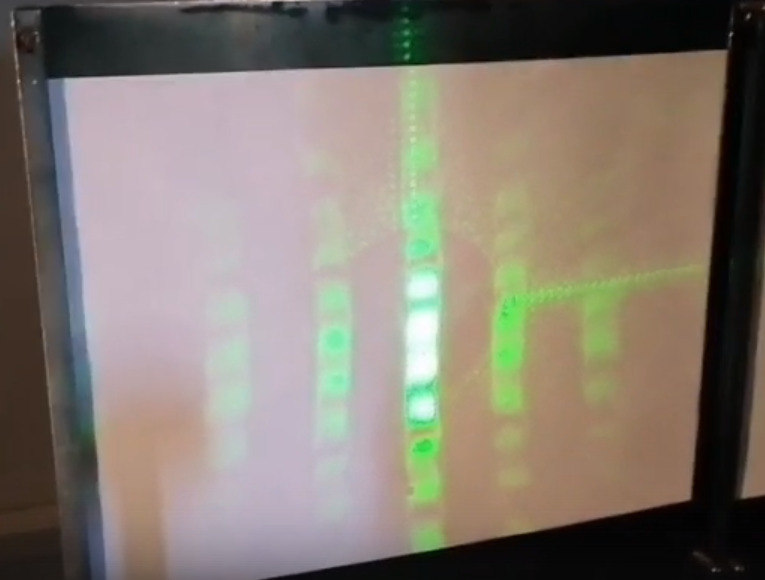
\includegraphics[width=1\textwidth]{Сетка4.png}
\end{center}
\caption{Сетка №4} \label{Сетка-4}
\end{figure}

\begin{figure}[h!]
\begin{center}
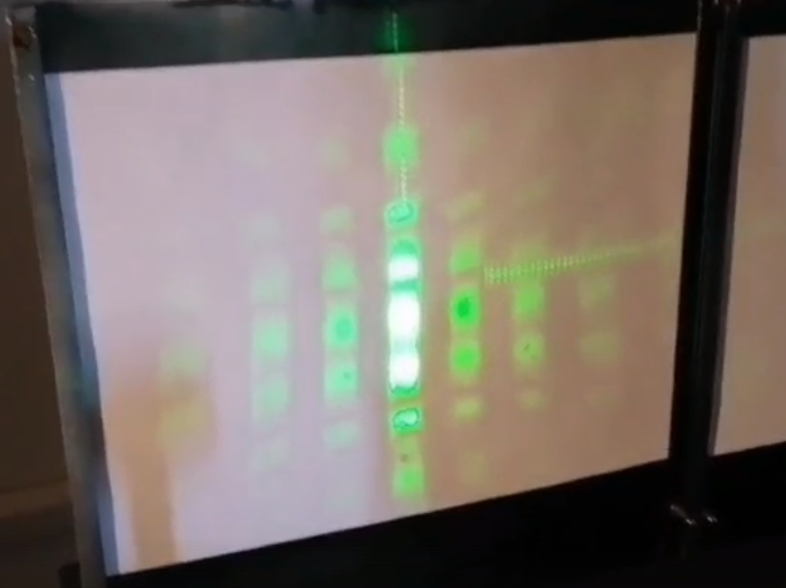
\includegraphics[width=1\textwidth]{Сетка5.png}
\end{center}
\caption{Сетка №5} \label{Сетка-5}
\end{figure}

\clearpage
При уменьшении периода сеток, период полосок на экране увеличивается.

~

2. Оставляем неизменной сетку №4, меняем размер щели диафрагмы:

\begin{figure}[h!]
\begin{center}
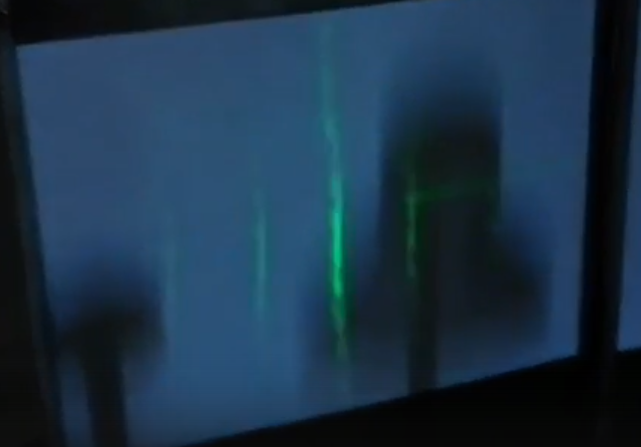
\includegraphics[width=1\textwidth]{Пост_сетка-1.png}
\end{center}
\caption{Изображение при увеличении щели} \label{Сетка4(1)}
\end{figure}

\clearpage
\begin{figure}[h!]
\begin{center}
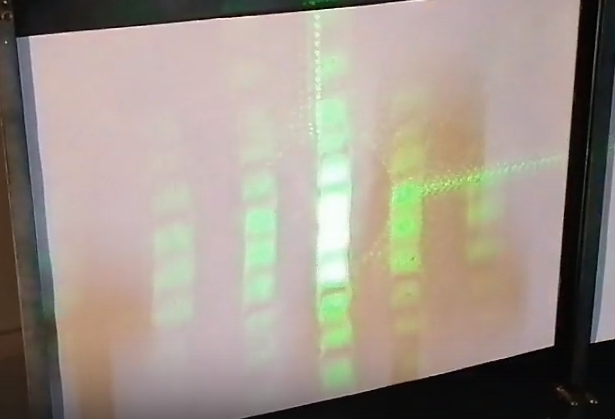
\includegraphics[width=1\textwidth]{Пост_сетка-2.png}
\end{center}
\caption{Изображение при уменьшении щели} \label{Сетка4(2)}
\end{figure}


При увеличении щели ширина полос уменьшается, при уменьшении -- наоборот увеличивается.

\section*{Выводы}

\begin{table}[h!]
\begin{tabular}{|l|lll|}
\hline
N сетки &  &                                 d, мкм                            &                         \\ \cline{2-4} 
        & \multicolumn{1}{l|}{Спектр}       & \multicolumn{1}{l|}{Микроскоп}   & Разрешающая способность \\ \hline
1       & \multicolumn{1}{l|}{$16,5 \pm 0,2$}   & \multicolumn{1}{l|}{$30,2 \pm 1,8$}  &                        \\ \hline
2       & \multicolumn{1}{l|}{$25,2 \pm 0,5$}   & \multicolumn{1}{l|}{$44,4 \pm 1,8$}  &                        \\ \hline
3       & \multicolumn{1}{l|}{$50,7 \pm 1,9$}   & \multicolumn{1}{l|}{$88,7 \pm 1,8$}  & $44,3 \pm 0,4$              \\ \hline
4       & \multicolumn{1}{l|}{$100,4 \pm 7,6$}  & \multicolumn{1}{l|}{$177,4 \pm 1,9$} & $79,2 \pm 1,2$             \\ \hline
5       & \multicolumn{1}{l|}{$136,4 \pm 13,9$} & \multicolumn{1}{l|}{$236 \pm 3,6$}   & $145,4 \pm 4$              \\ \hline
\end{tabular}
\end{table}

\end{document}